%%%%%%%%%%%%%%%%%%%%%%%%%%%%%%%%%%%%%%%%%%%%%%%%%%%%%%%%%%%%%%%%%%%%%%%%%%%%%%%%%%%%%%%%%%%%%%%%%%%%%%%%%%%%%%%%%%%%%%%%%%%%%%%%%%%%%%%%%%%%%%%%%%%%%%%%%%%%%%%%%%%
% Written By Michael Brodskiy
% Class: Fundamentals of Electronics
% Professor: M. Onabajo
%%%%%%%%%%%%%%%%%%%%%%%%%%%%%%%%%%%%%%%%%%%%%%%%%%%%%%%%%%%%%%%%%%%%%%%%%%%%%%%%%%%%%%%%%%%%%%%%%%%%%%%%%%%%%%%%%%%%%%%%%%%%%%%%%%%%%%%%%%%%%%%%%%%%%%%%%%%%%%%%%%%

\include{Includes.tex}

\title{Homework 11}
\date{\today}
\author{Michael Brodskiy\\ \small Professor: M. Onabajo}

\begin{document}

\maketitle

\begin{enumerate}

  \item
    
    \begin{enumerate}

      \item We may begin by saying that $V_{gs}(t)$ may be expressed as:

        $$V_{gs}(t)=V_{g}(t)-V_{s}(t)$$

        We may see that the source voltage is grounded, which lets us say:

        $$V_{gs}(t)=V_{g}(t)$$

        We may see that, taking the capacitor as a short, the voltage at $G$ is simply the sum of the input voltage and the divided voltage from the $20[\si{\volt}]$ supply voltage. Thus, we may write:

        $$V_g(t)=\frac{300k(20)}{300k+1700k}+V_i$$
        $$V_g(t)=3+\sin(2000\pi t)$$

        Thus, we may say:

        $$\boxed{V_{gs}(t)=3+\sin(2000\pi t)}$$

      \item Parts (b-d) are combined in the plot shown in (d)

      \item Parts (b-d) are combined in the plot shown in (d)

      \item We may generate the following plot:

        \begin{figure}[H]
          \centering
          \tikzset{every picture/.style={line width=0.75pt}} %set default line width to 0.75pt        

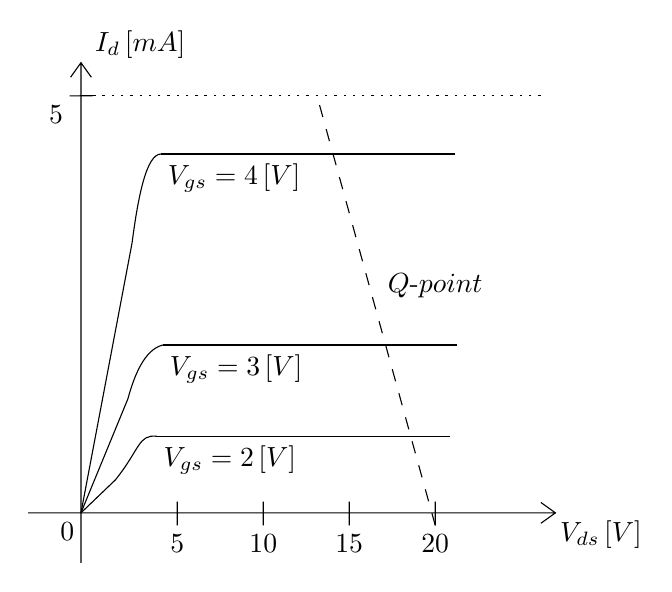
\begin{tikzpicture}[x=0.75pt,y=0.75pt,yscale=-1,xscale=1]
%uncomment if require: \path (0,300); %set diagram left start at 0, and has height of 300

%Shape: Axis 2D [id:dp7747432600161656] 
\draw  (212,239.9) -- (466,239.9)(237.4,23) -- (237.4,264) (459,234.9) -- (466,239.9) -- (459,244.9) (232.4,30) -- (237.4,23) -- (242.4,30)  ;
%Straight Lines [id:da32321167714042176] 
\draw    (232,39) -- (243.4,38.9) ;
%Straight Lines [id:da3826819041297148] 
\draw    (283.81,234.5) -- (283.82,245.9) ;
%Straight Lines [id:da8863803291808989] 
\draw    (325.23,234.5) -- (325.24,245.9) ;
%Straight Lines [id:da8836857250921787] 
\draw    (366.65,234.5) -- (366.66,245.9) ;
%Straight Lines [id:da6012153418314233] 
\draw    (408.08,234.5) -- (408.09,245.9) ;
%Straight Lines [id:da9669800699965388] 
\draw    (262,110) -- (237.4,239.9) ;
%Curve Lines [id:da052779219899400265] 
\draw    (262,110) .. controls (265,87) and (269,67) .. (276,67) ;
%Straight Lines [id:da3181020528582228] 
\draw    (417.42,67) -- (276,67) ;
%Straight Lines [id:da6235172620189178] 
\draw    (260,185) -- (237.4,239.9) ;
%Curve Lines [id:da5269697997504461] 
\draw    (260,185) .. controls (263,174) and (268,161) .. (277,159) ;
%Straight Lines [id:da8278207189697631] 
\draw    (418.42,159) -- (277,159) ;
%Straight Lines [id:da44370626554232584] 
\draw    (254,224) -- (237.4,239.9) ;
%Curve Lines [id:da5311110709342856] 
\draw    (254,224) .. controls (266,209) and (265,202) .. (274,203) ;
%Straight Lines [id:da3093865751796777] 
\draw    (415.42,203) -- (274,203) ;
%Straight Lines [id:da007117914624788946] 
\draw  [dash pattern={on 0.84pt off 2.51pt}]  (458.82,38.9) -- (243.4,38.9) ;
%Straight Lines [id:da5252561358577262] 
\draw  [dash pattern={on 4.5pt off 4.5pt}]  (408.09,245.9) -- (351.11,38.9) ;

% Text Node
\draw (243,6.4) node [anchor=north west][inner sep=0.75pt]    {$I_{d}\left[\text{mA}\right]$};
% Text Node
\draw (230,42.4) node [anchor=north east] [inner sep=0.75pt]    {$5$};
% Text Node
\draw (235.4,243.3) node [anchor=north east] [inner sep=0.75pt]    {$0$};
% Text Node
\draw (283.82,249.3) node [anchor=north] [inner sep=0.75pt]    {$5$};
% Text Node
\draw (325.24,249.3) node [anchor=north] [inner sep=0.75pt]    {$10$};
% Text Node
\draw (366.66,249.3) node [anchor=north] [inner sep=0.75pt]    {$15$};
% Text Node
\draw (408.09,249.3) node [anchor=north] [inner sep=0.75pt]    {$20$};
% Text Node
\draw (467,242.4) node [anchor=north west][inner sep=0.75pt]    {$V_{ds}\left[\text{V}\right]$};
% Text Node
\draw (278,70.4) node [anchor=north west][inner sep=0.75pt]    {$V_{gs} =4\left[\text{V}\right]$};
% Text Node
\draw (279,162.4) node [anchor=north west][inner sep=0.75pt]    {$V_{gs} =3\left[\text{V}\right]$};
% Text Node
\draw (276,206.4) node [anchor=north west][inner sep=0.75pt]    {$V_{gs} =2\left[\text{V}\right]$};
% Text Node
\draw (384,123.4) node [anchor=north west][inner sep=0.75pt]    {$Q\text{\mbox{-}point}$};


\end{tikzpicture}

          \caption{Plot for Parts (b)-(d)}
          \label{fig:1}
        \end{figure}

        We may observe, first and foremost, that the curve is zero for $V_{gs}=1[\si{\volt}]$, since, at this value, $V_{gs}=V_{to}$. We may observe via the load line in the plot that $V_{ds}\approx16[\si{\volt}]$ at the $Q$-point, and $V_{ds}^{max}\approx20[\si{\volt}]$ and $V_{ds}^{min}\approx10[\si{\volt}]$

    \end{enumerate}

  \item

    \begin{enumerate}

      \item We may observe that $V_1$ may be obtained using our equations:

        $$I_D=\frac{\mu_pC_{ox}W}{2L}[V_{GS}-|V_{t}|]^2$$
        $$8=.5[V_{GS}-|-1|]^2$$
        $$V_{GS}^2-2V_{GS}+1=16$$
        $$V_{GS}^2-2V_{GS}-15=0$$

        We see that the two solutions are $V_{GS}=5,-3[\si{\volt}]$. We know the value is positive, so we write:

        $$V_S-V_G=5$$
        $$V_G=V_S-5$$
        $$V_G=10-5$$
        $$\boxed{V_1=V_G=5[\si{\volt}]}$$

        We may then proceed to calculate the voltage using the current source, which is equal to $I_D$, at $V_2$, which we may find as:

        $$V_2=-10+8(.5)$$
        $$\boxed{V_2=-6[\si{\volt}]}$$

      \item From the figure, we may observe:

        $$V_3=V_{G1}$$
        $$V_S=15[\si{\volt}]$$

        We may use our formulas to write:

        $$I_D=\frac{\mu_p C_{ox}W}{2L}[V_{SG1}-|V_t|]^2$$

        Looking at the current source at the end, we see that $I_D=8[\si{\milli\ampere}]$. This lets us get:

        $$8=(.5)[V_{SG1}-|-1|]^2$$

        This lets us get (simplifying $V_{SG1}\to V$):

        $$V^2-2V+1=16$$
        $$V^2-2V-15=0$$
        $$(V-5)(V+3)=0$$
        $$V_{SG1}=5,-3$$

        We proceed with the positive value, which gives us:

        $$5=V_S-V_{G1}$$
        $$V_s-5=V_{G1}$$
        $$V_{G1}=15-5$$

        And finally:

        $$\boxed{V_3=V_{G1}=10[\si{\volt}]}$$

        We then use the same method to get $V_4=V_{G2}$:

        $$8=(.5)[V_{SG2}-|-1|]^2$$

        To simplify, take $V=V_{SG2}$:

        $$V^2-2V+1=16$$
        $$V=5,-3$$

        Again, we proceed with the positive value to get:

        $$V_{S}-V_{G2}=5$$
        $$V_{G2}=V_S-5$$
        $$V_{G2}=10-5$$

        This gets us:

        $$\boxed{V_4=V_{G2}=5[\si{\volt}]}$$

    \end{enumerate}

  \item

    \begin{enumerate}

      \item Taking the capacitors as open circuits, we end up with a circuit consisting solely of the $15[\si{\volt}]$ DC source, the NMOS, and the $10[\si{\mega\ohm}]$, $5[\si{\mega\ohm}]$, $7.5[\si{\kilo\ohm}]$, and $3[\si{\kilo\ohm}]$ resistors. This allows us to divide the voltage to find $V_G$:

        $$V_G=(V_{DC})\frac{5}{10+5}$$
        $$\boxed{V_G=5[\si{\volt}]}$$

        The drain current may be found as:

        $$I_D=\frac{V_S}{R_S}$$

        Alternatively, we may write:

        $$I_D=\frac{V_G-V_{GS}}{R_S}$$

        We can then equate this to our formula:

        $$I_D=K(V_{GS}-V_t)^2$$

        This gets us:

        $$V_{GS}^2-2V_{GS}+1=\frac{5-V_{GS}}{3}$$
        $$V_{GS}^2-\frac{5}{3}V_{GS}-\frac{2}{3}=$$
        $$V_{GS}=\frac{(5/3)\pm\sqrt{(25/9)-(4)(1)(-2/3)}}{2}$$
        $$V_{GS}=\frac{(5/3)\pm(7/3)}{2}$$
        $$V_{GS}=2,-\frac{1}{3}$$

        We proceed with the positive value:

        $$I_D=\frac{5-2}{3}[\si{\milli\ampere}]$$
        $$\boxed{I_D=1[\si{\milli\ampere}]}$$

        We may find the transconductance gain to get:

        $$g_m=\frac{2I_D}{V_{GS}-V_t}$$
        $$g_m=\frac{2(.001)}{2-1}$$
        $$\boxed{g_m=2[\si{\milli S}]}$$

        We can obtain:

        $$r_{ds}=\frac{V_A}{I_D}$$
        $$r_{ds}=\frac{100}{10^{-3}}$$
        $$\boxed{r_{ds}=100[\si{\kilo\ohm}]}$$

      \item 

      \item For the common source state, we know that $\boxed{Z_{in}\to\infty}$

      \item 

    \end{enumerate}

  \item

    \begin{enumerate}

      \item 

      \item 

      \item 

      \item 

    \end{enumerate}

\end{enumerate}

\end{document}

